\section{Gradient Descent} \label{sec:prob1}
In this section, we implemented Gradient Descent in Python to find the minimum of a function.

\subsection{Part 1}
Our Gradient Descent (GD) implementation begins with an initial guess, $x_0$, of the argument $x_{min}$ that minimizes the function, $f(x)$.
The implementation is applied to two functions, a negative Gaussian and a quadratic bowl.
The gradient, dfdx, can be calculated in closed form (for simple functions), and the next estimate of $x_{min}$ is updated according to the rule:
\begin{equation}
x_{i+1} = x_i - \alpha \cdot \frac{\partial f(x_i)}{\partial x}
\label{eq:gd}
\end{equation}
Here, $\alpha$ is the step size, or learning rate, which controls how much the gradient affects the next estimate.
The rule is applied until either a pre-determined maximum number of iterations, $n_{iters}$, occurs, or the function's value at the current iteration differs from the previous iteration's estimate by less than $\epsilon$.
Each of these paramters, ($\alpha$, $n_{iters}$, and $\epsilon$) impact the GD solution in different ways.

In~\cref{fig:initial_guess}, the intial guess, $x_0$, is varied to show that a close intial guess leads to convergence in only a few steps.
As the norm of difference between initial and final estimates grows, the number of iterations increases.
For certain initial guesses, we observed that the algorithm did not converge in some maximum number of iterations.
For the negative Gaussian, this is because the gradient is very small far from the mean.

The convergence limit determines when the GD algorithm stops, seen in ~\cref{fig:convergence}.
The error increases if $\epsilon$ is too large, as on the right of~\cref{fig:convergence1}.

In GD, the norm of the gradient decreases as the solution converges, which is shown for the quadratic bowl function in~\cref{fig:gradient}.


\begin{figure}
	\centering
	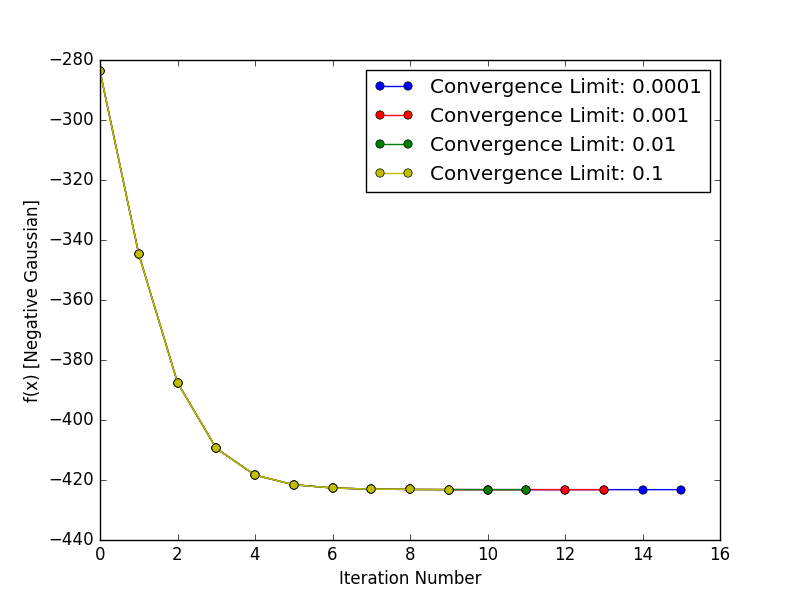
\includegraphics [trim=0 0 0 0, clip, angle=0, width=0.8\columnwidth,
	keepaspectratio]{figures/1_1_convergence1}
	\caption{As convergence limit, $\epsilon$, increases, the iteration stops earlier. From this view, the four solutions differ very little.} 
	\label{fig:convergence1} 
	%\vskip -0.1in
\end{figure}

\begin{figure}
	\centering
	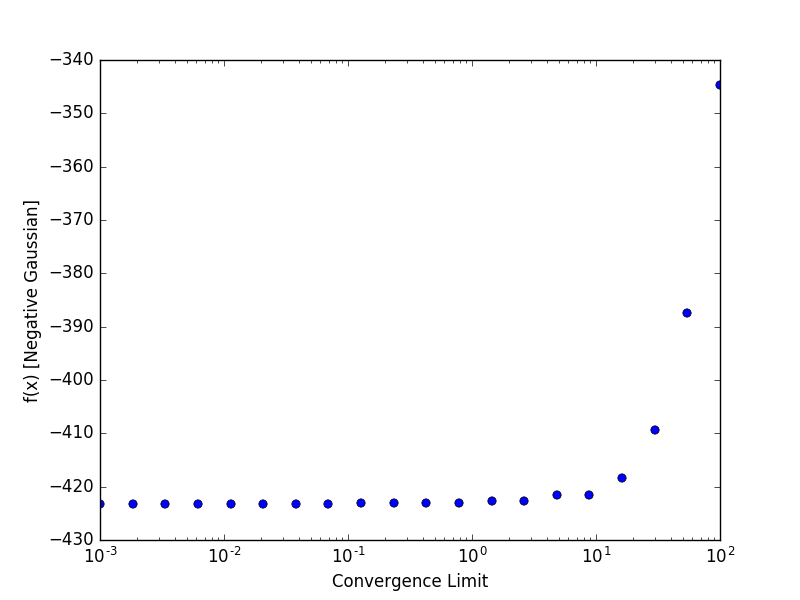
\includegraphics [trim=0 0 0 0, clip, angle=0, width=0.8\columnwidth,
	keepaspectratio]{figures/1_1_convergence}
	\caption{The final value returned by GD can differ substantially if convergence limit is set too loosely.} 
	\label{fig:convergence} 
	%\vskip -0.1in
\end{figure}

\begin{figure}
	\centering
	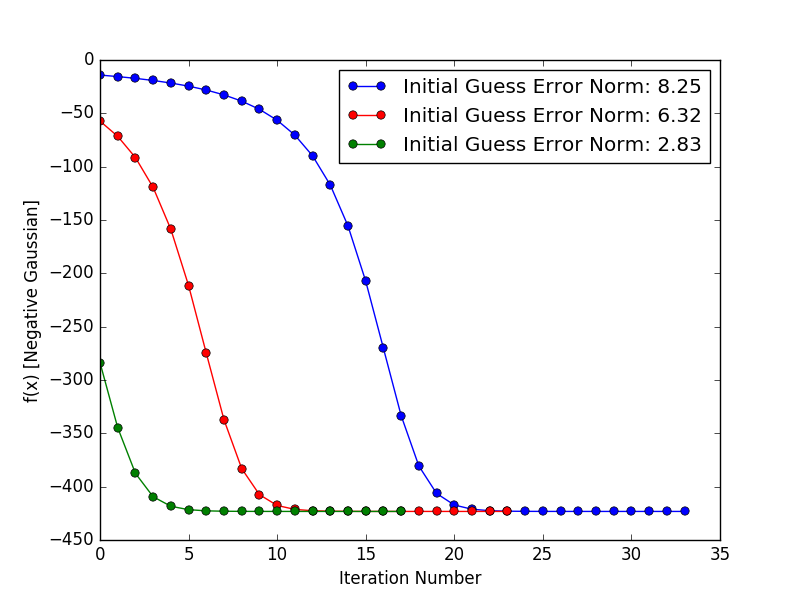
\includegraphics [trim=0 0 0 0, clip, angle=0, width=0.8\columnwidth,
	keepaspectratio]{figures/1_1_initial_guess}
	\caption{When initial guess is far from true minimum, it takes many iterations (blue) to converge. As initial guess approaches final solution, number of iterations decreases.} 
	\label{fig:initial_guess} 
	%\vskip -0.1in
\end{figure}

\begin{figure}
	\centering
	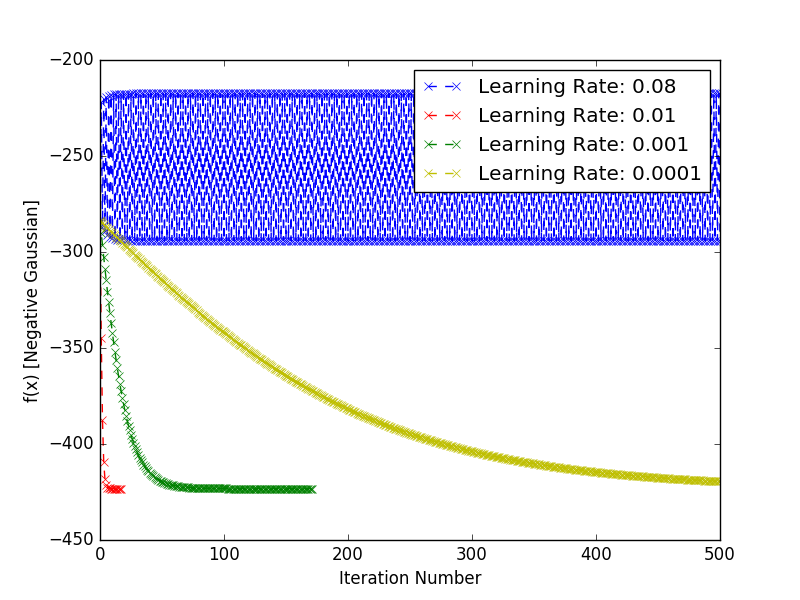
\includegraphics [trim=0 0 0 0, clip, angle=0, width=0.8\columnwidth,
	keepaspectratio]{figures/1_1_step_size}
	\caption{If learning rate, $\alpha$, is too large (blue), the solution will oscillate or diverge each iteration. If $\alpha$ is too small, it will take many iterations to converge (yellow). Convergence takes only a few iterations for proper $\alpha$ (red).} 
	\label{fig:learning_rate} 
	%\vskip -0.1in
\end{figure}

\begin{figure}
	\centering
	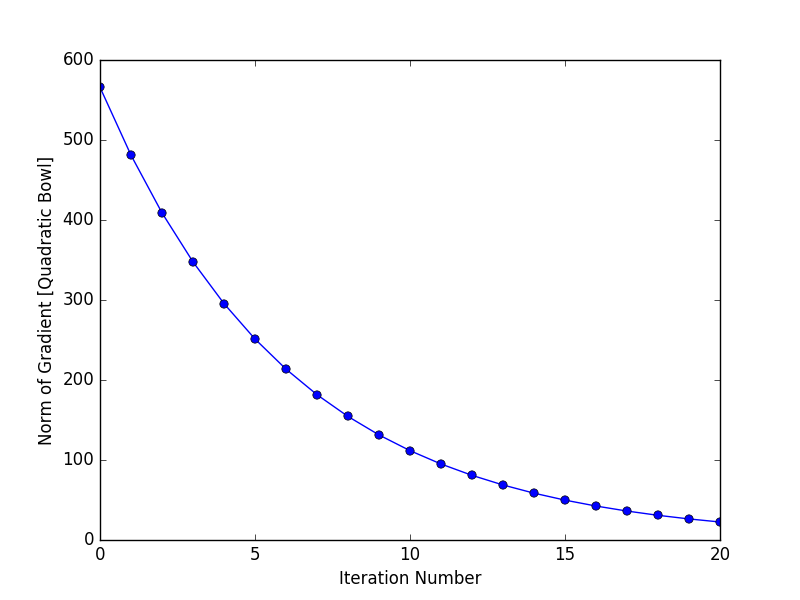
\includegraphics [trim=0 0 0 0, clip, angle=0, width=0.8\columnwidth,
	keepaspectratio]{figures/1_1_gradient}
	\caption{Norm of gradient decreases with each iteration in GD. This example minimizes the Quadratic Bowl function.} 
	\label{fig:gradient} 
	%\vskip -0.1in
\end{figure}


\subsection{Part 2}
For more complicated functions, the gradient is not always as easy to compute.
Instead, we can use finite difference approximation instead of a the closed form gradient.
The gradient approximation for a function of two variables is:
\begin{equation}
\nabla f = \begin{bmatrix}
	f_x & f_y
\end{bmatrix}
\approx \begin{bmatrix}
	\frac{f(x+\delta x, y) - f(x,y)}{\delta x} & \frac{f(x, y+\delta y) - f(x,y)}{\delta y}
\end{bmatrix}
\end{equation}

\begin{table*}[t]
  \centering
  \caption[]{Gradient vs. Finite Difference (Negative Gaussian and Quadratic Bowl)}
	\begin{tabular}{|p{3cm}||p{3cm}|p{3cm}|p{3cm}|p{3cm}|}
	 \hline
	 \multicolumn{5}{|c|}{Gradient vs Finite Difference ($\delta x = 0.01$)} \\
	 \hline
	 Function & Gradient & Approximation & Error &Error Norm \\
	 \hline
	 Neg. Gaussian: $f(3,4)$ & [-4.2258, -3.6221] & [-4.2375, -3.6299] & [-0.01178, -0.00785] & 0.0141 \\
	 Neg. Gaussian: $f(12,4)$ & [ 11.455, -34.365,] & [ 11.472, -34.440,] & [ 0.017, -0.074, ] & 0.0764 \\
	 Quad. Bowl: $f(6,2)$ & [-330, -350] & [-329.95, -349.95] & [ 0.05  0.05] & 0.0707\\
	 Quad. Bowl: $f(10^3,90)$ & [ 10050, 5500] & [ 10050.05, 5500.05] & [ 0.05, 0.05] & 0.0707 \\
	 \hline
	\end{tabular}
\end{table*}\label{table:gradient}

\begin{figure}
	\centering
	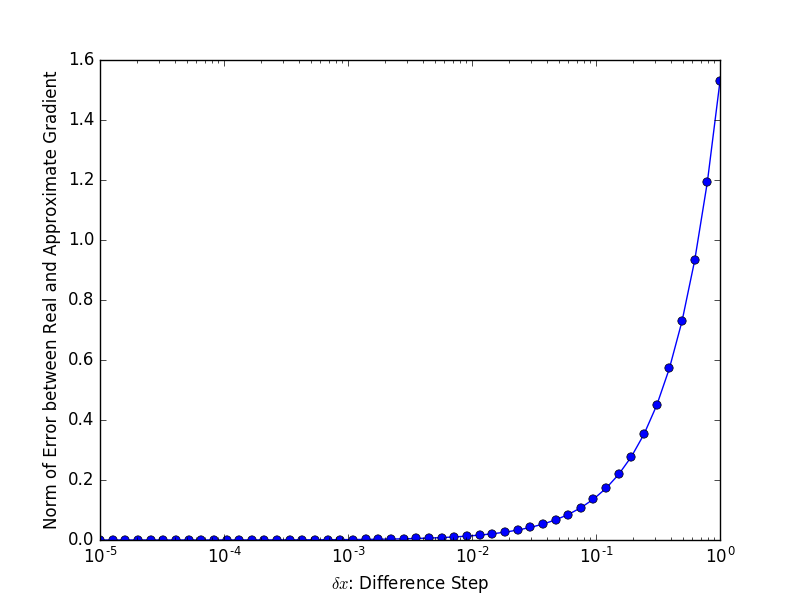
\includegraphics [trim=0 0 0 0, clip, angle=0, width=0.8\columnwidth,
	keepaspectratio]{figures/1_2_error}
	\caption{Norm of gradient approximation error increases as $\delta x$ increases. This plot is for the Negative Gaussian evaluated at (3,4).} 
	\label{fig:1_2_error} 
	%\vskip -0.1in
\end{figure}

While~\cref{table:gradient} shows that the error is rather small across a range of (x,y) values for the two functions, the choice of difference step $\delta x$ is what led to this small error. In~\cref{fig:1_2_error}, the norm of the difference between the real and approximate gradient gets quite large when $\delta x$ is also large.


\subsection{Part 3}
Next, we consider two types of gradient descent on a dataset.
Batch gradient descent (GD) calculates the gradient at each step using every sample in the data set.
Stochastic gradient descent (SGD), instead uses a single sample each iteration, looping through a random ordering of the dataset to add a stochastic element.
We implemented both algorithms and evaluated them on the same data set, with the same initial guess.
For SGD, the equation~\cref{eq:gd} is modified to accept a single sample, $(x^j,y^j)$ as input to the gradient:
\begin{equation}
\theta_{i+1} = \theta_i - \eta_i \cdot \nabla_\theta J(\theta_i;x^{(j)},y^{(j)})
\label{eq:sgd}
\end{equation}
We use a common form of learning rate parameter $\eta_i = (\tau_0+i)^{-k}$ to guarantee convergence with $\tau_0=10^8$ and $k=0.6$.

In~\cref{fig:1_3_sgd_early}, Stochastic Gradient Descent (green) initially approaches convergence faster than Batch Gradient Descent (blue).
Batch GD monotonically decreases in norm error, but SGD randomly oscillates and sometimes increases.
Batch GD looks piecewise linear, because each iteration involves 100 (size of dataset) evaluations of the gradient, whereas SGD only evaluates once per iteration.
So, SGD intially learns faster than Batch GD.

After many iterations~\cref{fig:1_3_sgd_late}, Batch Gradient Descent catches up to Stochastic Gradient Descent and is more accurate.
SGD seems to converge within a range, but continues to oscillate as long as learning rate is non-zero.
So, Batch GD has better accuracy than SGD.
The tradeoff here is speed vs. accuracy.


\begin{figure}
	\centering
	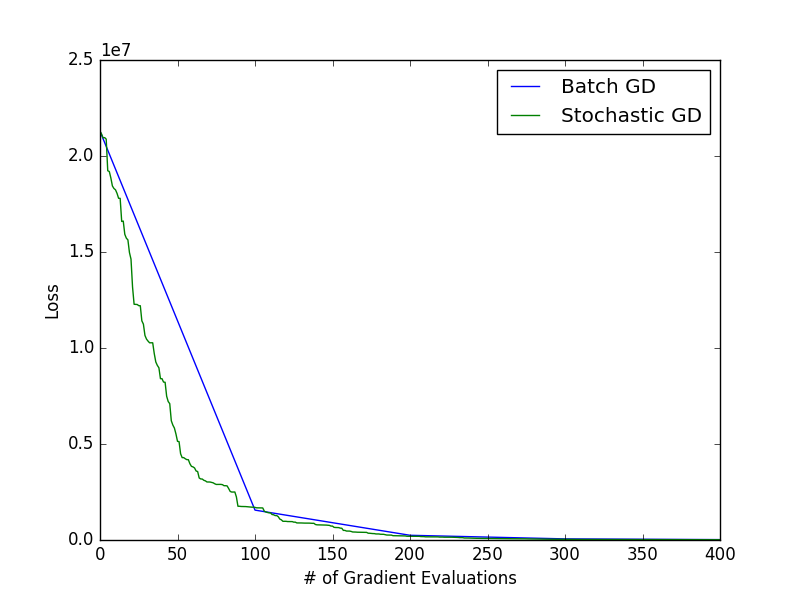
\includegraphics [trim=0 0 0 0, clip, angle=0, width=0.8\columnwidth,
	keepaspectratio]{figures/1_3_sgd_early}
	\caption{Stochastic Gradient Descent (green) initially approaches convergence faster than Batch Gradient Descent (blue). Batch GD monotonically decreases in norm error, but SGD randomly oscillates and sometimes increases. Batch GD looks piecewise linear, because each iteration involves 100 (size of dataset) evaluations of the gradient, whereas SGD only evaluates once per iteration.} 
	\label{fig:1_3_sgd_early} 
	%\vskip -0.1in
\end{figure}

\begin{figure}
	\centering
	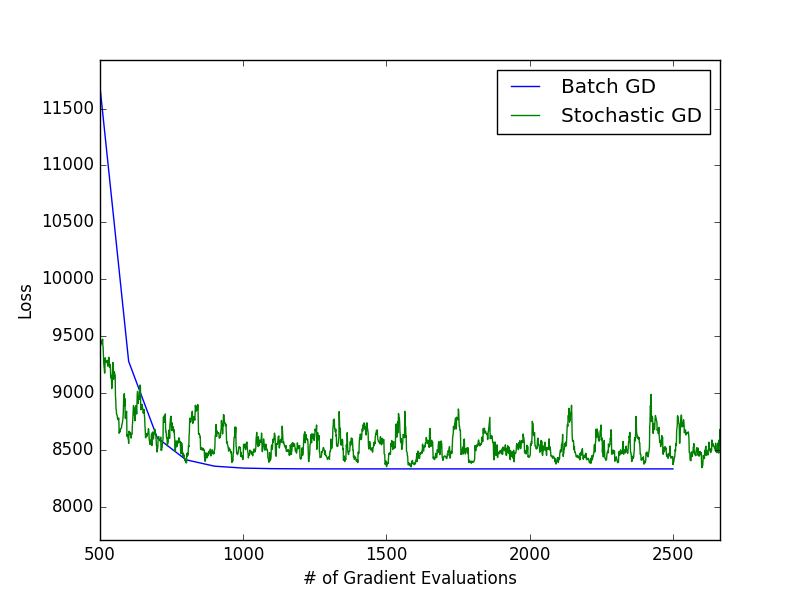
\includegraphics [trim=0 0 0 0, clip, angle=0, width=0.8\columnwidth,
	keepaspectratio]{figures/1_3_sgd_late}
	\caption{After many iterations, Batch Gradient Descent catches up to Stochastic Gradient Descent and is more accurate. SGD seems to converge within a range, but continues to oscillate as long as learning rate is non-zero.} 
	\label{fig:1_3_sgd_late} 
	%\vskip -0.1in
\end{figure}









